\documentclass[twoside]{book}

% Packages required by doxygen
\usepackage{fixltx2e}
\usepackage{calc}
\usepackage{doxygen}
\usepackage[export]{adjustbox} % also loads graphicx
\usepackage{graphicx}
\usepackage[utf8]{inputenc}
\usepackage{makeidx}
\usepackage{multicol}
\usepackage{multirow}
\PassOptionsToPackage{warn}{textcomp}
\usepackage{textcomp}
\usepackage[nointegrals]{wasysym}
\usepackage[table]{xcolor}

% Font selection
\usepackage[T1]{fontenc}
\usepackage[scaled=.90]{helvet}
\usepackage{courier}
\usepackage{amssymb}
\usepackage{sectsty}
\renewcommand{\familydefault}{\sfdefault}
\allsectionsfont{%
  \fontseries{bc}\selectfont%
  \color{darkgray}%
}
\renewcommand{\DoxyLabelFont}{%
  \fontseries{bc}\selectfont%
  \color{darkgray}%
}
\newcommand{\+}{\discretionary{\mbox{\scriptsize$\hookleftarrow$}}{}{}}

% Page & text layout
\usepackage{geometry}
\geometry{%
  a4paper,%
  top=2.5cm,%
  bottom=2.5cm,%
  left=2.5cm,%
  right=2.5cm%
}
\tolerance=750
\hfuzz=15pt
\hbadness=750
\setlength{\emergencystretch}{15pt}
\setlength{\parindent}{0cm}
\setlength{\parskip}{3ex plus 2ex minus 2ex}
\makeatletter
\renewcommand{\paragraph}{%
  \@startsection{paragraph}{4}{0ex}{-1.0ex}{1.0ex}{%
    \normalfont\normalsize\bfseries\SS@parafont%
  }%
}
\renewcommand{\subparagraph}{%
  \@startsection{subparagraph}{5}{0ex}{-1.0ex}{1.0ex}{%
    \normalfont\normalsize\bfseries\SS@subparafont%
  }%
}
\makeatother

% Headers & footers
\usepackage{fancyhdr}
\pagestyle{fancyplain}
\fancyhead[LE]{\fancyplain{}{\bfseries\thepage}}
\fancyhead[CE]{\fancyplain{}{}}
\fancyhead[RE]{\fancyplain{}{\bfseries\leftmark}}
\fancyhead[LO]{\fancyplain{}{\bfseries\rightmark}}
\fancyhead[CO]{\fancyplain{}{}}
\fancyhead[RO]{\fancyplain{}{\bfseries\thepage}}
\fancyfoot[LE]{\fancyplain{}{}}
\fancyfoot[CE]{\fancyplain{}{}}
\fancyfoot[RE]{\fancyplain{}{\bfseries\scriptsize Generated by Doxygen }}
\fancyfoot[LO]{\fancyplain{}{\bfseries\scriptsize Generated by Doxygen }}
\fancyfoot[CO]{\fancyplain{}{}}
\fancyfoot[RO]{\fancyplain{}{}}
\renewcommand{\footrulewidth}{0.4pt}
\renewcommand{\chaptermark}[1]{%
  \markboth{#1}{}%
}
\renewcommand{\sectionmark}[1]{%
  \markright{\thesection\ #1}%
}

% Indices & bibliography
\usepackage{natbib}
\usepackage[titles]{tocloft}
\setcounter{tocdepth}{3}
\setcounter{secnumdepth}{5}
\makeindex

% Hyperlinks (required, but should be loaded last)
\usepackage{ifpdf}
\ifpdf
  \usepackage[pdftex,pagebackref=true]{hyperref}
\else
  \usepackage[ps2pdf,pagebackref=true]{hyperref}
\fi
\hypersetup{%
  colorlinks=true,%
  linkcolor=blue,%
  citecolor=blue,%
  unicode%
}

% Custom commands
\newcommand{\clearemptydoublepage}{%
  \newpage{\pagestyle{empty}\cleardoublepage}%
}

\usepackage{caption}
\captionsetup{labelsep=space,justification=centering,font={bf},singlelinecheck=off,skip=4pt,position=top}

%===== C O N T E N T S =====

\begin{document}

% Titlepage & ToC
\hypersetup{pageanchor=false,
             bookmarksnumbered=true,
             pdfencoding=unicode
            }
\pagenumbering{roman}
\begin{titlepage}
\vspace*{7cm}
\begin{center}%
{\Large Project X Ecobot }\\
\vspace*{1cm}
{\large Generated by Doxygen 1.8.11}\\
\end{center}
\end{titlepage}
\clearemptydoublepage
\tableofcontents
\clearemptydoublepage
\pagenumbering{arabic}
\hypersetup{pageanchor=true}

%--- Begin generated contents ---
\chapter{Hierarchical Index}
\section{Class Hierarchy}
This inheritance list is sorted roughly, but not completely, alphabetically\+:\begin{DoxyCompactList}
\item \contentsline{section}{Image\+Analysis}{\pageref{classImageAnalysis}}{}
\item \contentsline{section}{I\+Planning\+Alg}{\pageref{classIPlanningAlg}}{}
\begin{DoxyCompactList}
\item \contentsline{section}{Greedy\+Alg}{\pageref{classGreedyAlg}}{}
\item \contentsline{section}{Low\+X\+Alg}{\pageref{classLowXAlg}}{}
\end{DoxyCompactList}
\item \contentsline{section}{Point}{\pageref{classPoint}}{}
\item \contentsline{section}{State\+Machine}{\pageref{classStateMachine}}{}
\end{DoxyCompactList}

\chapter{Class Index}
\section{Class List}
Here are the classes, structs, unions and interfaces with brief descriptions\+:\begin{DoxyCompactList}
\item\contentsline{section}{\hyperlink{classGreedyAlg}{Greedy\+Alg} }{\pageref{classGreedyAlg}}{}
\item\contentsline{section}{\hyperlink{classImageAnalysis}{Image\+Analysis} }{\pageref{classImageAnalysis}}{}
\item\contentsline{section}{\hyperlink{classIPlanningAlg}{I\+Planning\+Alg} }{\pageref{classIPlanningAlg}}{}
\item\contentsline{section}{\hyperlink{classLowXAlg}{Low\+X\+Alg} }{\pageref{classLowXAlg}}{}
\item\contentsline{section}{\hyperlink{classPoint}{Point} }{\pageref{classPoint}}{}
\item\contentsline{section}{\hyperlink{classStateMachine}{State\+Machine} }{\pageref{classStateMachine}}{}
\end{DoxyCompactList}

\chapter{File Index}
\section{File List}
Here is a list of all files with brief descriptions\+:\begin{DoxyCompactList}
\item\contentsline{section}{/home/lydiazoghbi/catkin\+\_\+ws/src/project\+\_\+x\+\_\+ecobot/include/\hyperlink{GreedyAlg_8hpp}{Greedy\+Alg.\+hpp} \\*Header file for \hyperlink{classGreedyAlg}{Greedy\+Alg} class }{\pageref{GreedyAlg_8hpp}}{}
\item\contentsline{section}{/home/lydiazoghbi/catkin\+\_\+ws/src/project\+\_\+x\+\_\+ecobot/include/\hyperlink{ImageAnalysis_8hpp}{Image\+Analysis.\+hpp} \\*Header file for \hyperlink{classImageAnalysis}{Image\+Analysis} class }{\pageref{ImageAnalysis_8hpp}}{}
\item\contentsline{section}{/home/lydiazoghbi/catkin\+\_\+ws/src/project\+\_\+x\+\_\+ecobot/include/\hyperlink{IPlanningAlg_8hpp}{I\+Planning\+Alg.\+hpp} }{\pageref{IPlanningAlg_8hpp}}{}
\item\contentsline{section}{/home/lydiazoghbi/catkin\+\_\+ws/src/project\+\_\+x\+\_\+ecobot/include/\hyperlink{LowXAlg_8hpp}{Low\+X\+Alg.\+hpp} \\*Header file for \hyperlink{classLowXAlg}{Low\+X\+Alg} class }{\pageref{LowXAlg_8hpp}}{}
\item\contentsline{section}{/home/lydiazoghbi/catkin\+\_\+ws/src/project\+\_\+x\+\_\+ecobot/include/\hyperlink{Point_8hpp}{Point.\+hpp} \\*Header file for \hyperlink{IPlanningAlg_8hpp}{I\+Planning\+Alg.\+hpp} }{\pageref{Point_8hpp}}{}
\item\contentsline{section}{/home/lydiazoghbi/catkin\+\_\+ws/src/project\+\_\+x\+\_\+ecobot/include/\hyperlink{StateMachine_8hpp}{State\+Machine.\+hpp} \\*Header file for \hyperlink{classStateMachine}{State\+Machine} class }{\pageref{StateMachine_8hpp}}{}
\end{DoxyCompactList}

\chapter{Class Documentation}
\hypertarget{classGreedyAlg}{}\section{Greedy\+Alg Class Reference}
\label{classGreedyAlg}\index{Greedy\+Alg@{Greedy\+Alg}}


{\ttfamily \#include $<$Greedy\+Alg.\+hpp$>$}



Inheritance diagram for Greedy\+Alg\+:
\nopagebreak
\begin{figure}[H]
\begin{center}
\leavevmode
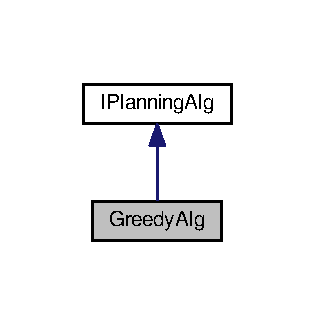
\includegraphics[width=151pt]{classGreedyAlg__inherit__graph}
\end{center}
\end{figure}


Collaboration diagram for Greedy\+Alg\+:
\nopagebreak
\begin{figure}[H]
\begin{center}
\leavevmode
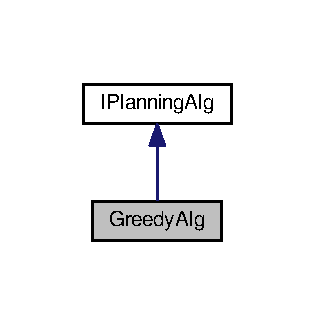
\includegraphics[width=151pt]{classGreedyAlg__coll__graph}
\end{center}
\end{figure}
\subsection*{Public Member Functions}
\begin{DoxyCompactItemize}
\item 
\hyperlink{classGreedyAlg_acd3e65e201585039b6d5135d8a75fe24}{$\sim$\+Greedy\+Alg} ()
\begin{DoxyCompactList}\small\item\em Destructor for the \hyperlink{classGreedyAlg}{Greedy\+Alg} class. \end{DoxyCompactList}\item 
void \hyperlink{classGreedyAlg_a5048e07294c60d726fdd7c82f0647dc6}{create\+Plan} (\hyperlink{classPoint}{Point} robot\+Location)
\begin{DoxyCompactList}\small\item\em Plan creation for how to pick up the debris. \end{DoxyCompactList}\item 
void \hyperlink{classGreedyAlg_a4ce065242ae545ec81ea4599c3b5fcdd}{push} (\hyperlink{classPoint}{Point} debris\+Location)
\begin{DoxyCompactList}\small\item\em Function for adding the debris into a debris vector. \end{DoxyCompactList}\item 
\hyperlink{classPoint}{Point} \hyperlink{classGreedyAlg_a72f7ee716b3c2010070e0f729780d203}{pop} (\hyperlink{classPoint}{Point} robot\+Location)
\begin{DoxyCompactList}\small\item\em Function for extracting the debris on the top of the vector. \end{DoxyCompactList}\end{DoxyCompactItemize}


\subsection{Constructor \& Destructor Documentation}
\index{Greedy\+Alg@{Greedy\+Alg}!````~Greedy\+Alg@{$\sim$\+Greedy\+Alg}}
\index{````~Greedy\+Alg@{$\sim$\+Greedy\+Alg}!Greedy\+Alg@{Greedy\+Alg}}
\subsubsection[{\texorpdfstring{$\sim$\+Greedy\+Alg()}{~GreedyAlg()}}]{\setlength{\rightskip}{0pt plus 5cm}Greedy\+Alg\+::$\sim$\+Greedy\+Alg (
\begin{DoxyParamCaption}
{}
\end{DoxyParamCaption}
)}\hypertarget{classGreedyAlg_acd3e65e201585039b6d5135d8a75fe24}{}\label{classGreedyAlg_acd3e65e201585039b6d5135d8a75fe24}


Destructor for the \hyperlink{classGreedyAlg}{Greedy\+Alg} class. 


\begin{DoxyParams}{Parameters}
{\em None} & \\
\hline
\end{DoxyParams}
\begin{DoxyReturn}{Returns}
None 
\end{DoxyReturn}


\subsection{Member Function Documentation}
\index{Greedy\+Alg@{Greedy\+Alg}!create\+Plan@{create\+Plan}}
\index{create\+Plan@{create\+Plan}!Greedy\+Alg@{Greedy\+Alg}}
\subsubsection[{\texorpdfstring{create\+Plan(\+Point robot\+Location)}{createPlan(Point robotLocation)}}]{\setlength{\rightskip}{0pt plus 5cm}void Greedy\+Alg\+::create\+Plan (
\begin{DoxyParamCaption}
\item[{{\bf Point}}]{robot\+Location}
\end{DoxyParamCaption}
)\hspace{0.3cm}{\ttfamily [virtual]}}\hypertarget{classGreedyAlg_a5048e07294c60d726fdd7c82f0647dc6}{}\label{classGreedyAlg_a5048e07294c60d726fdd7c82f0647dc6}


Plan creation for how to pick up the debris. 


\begin{DoxyParams}{Parameters}
{\em Robot\textquotesingle{}s} & current (x,y) location \\
\hline
\end{DoxyParams}
\begin{DoxyReturn}{Returns}
None 
\end{DoxyReturn}


Implements \hyperlink{classIPlanningAlg_abae4e6198042e0acf9abec46e624cd14}{I\+Planning\+Alg}.

\index{Greedy\+Alg@{Greedy\+Alg}!pop@{pop}}
\index{pop@{pop}!Greedy\+Alg@{Greedy\+Alg}}
\subsubsection[{\texorpdfstring{pop(\+Point robot\+Location)}{pop(Point robotLocation)}}]{\setlength{\rightskip}{0pt plus 5cm}{\bf Point} Greedy\+Alg\+::pop (
\begin{DoxyParamCaption}
\item[{{\bf Point}}]{robot\+Location}
\end{DoxyParamCaption}
)\hspace{0.3cm}{\ttfamily [virtual]}}\hypertarget{classGreedyAlg_a72f7ee716b3c2010070e0f729780d203}{}\label{classGreedyAlg_a72f7ee716b3c2010070e0f729780d203}


Function for extracting the debris on the top of the vector. 


\begin{DoxyParams}{Parameters}
{\em Robot\textquotesingle{}s} & current (x,y) location \\
\hline
\end{DoxyParams}
\begin{DoxyReturn}{Returns}
Position of debris 
\end{DoxyReturn}


Implements \hyperlink{classIPlanningAlg_a4f881df301b194754b1b81ddccad1ed4}{I\+Planning\+Alg}.

\index{Greedy\+Alg@{Greedy\+Alg}!push@{push}}
\index{push@{push}!Greedy\+Alg@{Greedy\+Alg}}
\subsubsection[{\texorpdfstring{push(\+Point debris\+Location)}{push(Point debrisLocation)}}]{\setlength{\rightskip}{0pt plus 5cm}void Greedy\+Alg\+::push (
\begin{DoxyParamCaption}
\item[{{\bf Point}}]{debris\+Location}
\end{DoxyParamCaption}
)\hspace{0.3cm}{\ttfamily [virtual]}}\hypertarget{classGreedyAlg_a4ce065242ae545ec81ea4599c3b5fcdd}{}\label{classGreedyAlg_a4ce065242ae545ec81ea4599c3b5fcdd}


Function for adding the debris into a debris vector. 


\begin{DoxyParams}{Parameters}
{\em Observed} & debris location \\
\hline
\end{DoxyParams}
\begin{DoxyReturn}{Returns}
None 
\end{DoxyReturn}


Implements \hyperlink{classIPlanningAlg_a2bda969cf89a041cb9fbbc7574e7b94f}{I\+Planning\+Alg}.



The documentation for this class was generated from the following file\+:\begin{DoxyCompactItemize}
\item 
/home/lydiazoghbi/catkin\+\_\+ws/src/project\+\_\+x\+\_\+ecobot/include/\hyperlink{GreedyAlg_8hpp}{Greedy\+Alg.\+hpp}\end{DoxyCompactItemize}

\hypertarget{classImageAnalysis}{}\section{Image\+Analysis Class Reference}
\label{classImageAnalysis}\index{Image\+Analysis@{Image\+Analysis}}


{\ttfamily \#include $<$Image\+Analysis.\+hpp$>$}

\subsection*{Public Member Functions}
\begin{DoxyCompactItemize}
\item 
\hyperlink{classImageAnalysis_a9a05460445d26581927b73f26b454db1}{Image\+Analysis} ()
\begin{DoxyCompactList}\small\item\em Constructor for \hyperlink{classImageAnalysis}{Image\+Analysis} class. \end{DoxyCompactList}\item 
double \hyperlink{classImageAnalysis_a71f0d5076443121ea81c7142e854cb32}{get\+Rotation\+Angle} (double current\+Orientation, double current\+Distance)
\begin{DoxyCompactList}\small\item\em Obtaining the angle by which the robot should rotate. \end{DoxyCompactList}\item 
cv\+::\+Mat \hyperlink{classImageAnalysis_ad138d68fd0f31fa0e896321d56a4d7e0}{filter} (cv\+::\+Mat raw\+Image)
\begin{DoxyCompactList}\small\item\em Filter function using H\+SV. \end{DoxyCompactList}\item 
void \hyperlink{classImageAnalysis_a8bab2847e38371a8a0bbeb7a4ae46dd8}{detect\+Debris} (cv\+::\+Mat filtered\+Image)
\begin{DoxyCompactList}\small\item\em Debris detection function. \end{DoxyCompactList}\item 
\hyperlink{classPoint}{Point} \hyperlink{classImageAnalysis_aedf9a6a46c20c2dc01579d80df30ee7e}{get\+Debris\+Image\+Location} ()
\begin{DoxyCompactList}\small\item\em Getter function. \end{DoxyCompactList}\end{DoxyCompactItemize}


\subsection{Constructor \& Destructor Documentation}
\index{Image\+Analysis@{Image\+Analysis}!Image\+Analysis@{Image\+Analysis}}
\index{Image\+Analysis@{Image\+Analysis}!Image\+Analysis@{Image\+Analysis}}
\subsubsection[{\texorpdfstring{Image\+Analysis()}{ImageAnalysis()}}]{\setlength{\rightskip}{0pt plus 5cm}Image\+Analysis\+::\+Image\+Analysis (
\begin{DoxyParamCaption}
{}
\end{DoxyParamCaption}
)}\hypertarget{classImageAnalysis_a9a05460445d26581927b73f26b454db1}{}\label{classImageAnalysis_a9a05460445d26581927b73f26b454db1}


Constructor for \hyperlink{classImageAnalysis}{Image\+Analysis} class. 


\begin{DoxyParams}{Parameters}
{\em None} & \\
\hline
\end{DoxyParams}
\begin{DoxyReturn}{Returns}
None 
\end{DoxyReturn}


\subsection{Member Function Documentation}
\index{Image\+Analysis@{Image\+Analysis}!detect\+Debris@{detect\+Debris}}
\index{detect\+Debris@{detect\+Debris}!Image\+Analysis@{Image\+Analysis}}
\subsubsection[{\texorpdfstring{detect\+Debris(cv\+::\+Mat filtered\+Image)}{detectDebris(cv::Mat filteredImage)}}]{\setlength{\rightskip}{0pt plus 5cm}void Image\+Analysis\+::detect\+Debris (
\begin{DoxyParamCaption}
\item[{cv\+::\+Mat}]{filtered\+Image}
\end{DoxyParamCaption}
)}\hypertarget{classImageAnalysis_a8bab2847e38371a8a0bbeb7a4ae46dd8}{}\label{classImageAnalysis_a8bab2847e38371a8a0bbeb7a4ae46dd8}


Debris detection function. 


\begin{DoxyParams}{Parameters}
{\em Filtered} & image using H\+SV \\
\hline
\end{DoxyParams}
\begin{DoxyReturn}{Returns}
None 
\end{DoxyReturn}
\index{Image\+Analysis@{Image\+Analysis}!filter@{filter}}
\index{filter@{filter}!Image\+Analysis@{Image\+Analysis}}
\subsubsection[{\texorpdfstring{filter(cv\+::\+Mat raw\+Image)}{filter(cv::Mat rawImage)}}]{\setlength{\rightskip}{0pt plus 5cm}cv\+::\+Mat Image\+Analysis\+::filter (
\begin{DoxyParamCaption}
\item[{cv\+::\+Mat}]{raw\+Image}
\end{DoxyParamCaption}
)}\hypertarget{classImageAnalysis_ad138d68fd0f31fa0e896321d56a4d7e0}{}\label{classImageAnalysis_ad138d68fd0f31fa0e896321d56a4d7e0}


Filter function using H\+SV. 


\begin{DoxyParams}{Parameters}
{\em R\+GB} & image \\
\hline
\end{DoxyParams}
\begin{DoxyReturn}{Returns}
Filtered image 
\end{DoxyReturn}
\index{Image\+Analysis@{Image\+Analysis}!get\+Debris\+Image\+Location@{get\+Debris\+Image\+Location}}
\index{get\+Debris\+Image\+Location@{get\+Debris\+Image\+Location}!Image\+Analysis@{Image\+Analysis}}
\subsubsection[{\texorpdfstring{get\+Debris\+Image\+Location()}{getDebrisImageLocation()}}]{\setlength{\rightskip}{0pt plus 5cm}{\bf Point} Image\+Analysis\+::get\+Debris\+Image\+Location (
\begin{DoxyParamCaption}
{}
\end{DoxyParamCaption}
)}\hypertarget{classImageAnalysis_aedf9a6a46c20c2dc01579d80df30ee7e}{}\label{classImageAnalysis_aedf9a6a46c20c2dc01579d80df30ee7e}


Getter function. 


\begin{DoxyParams}{Parameters}
{\em None} & \\
\hline
\end{DoxyParams}
\begin{DoxyReturn}{Returns}
Position of debris in image frame 
\end{DoxyReturn}
\index{Image\+Analysis@{Image\+Analysis}!get\+Rotation\+Angle@{get\+Rotation\+Angle}}
\index{get\+Rotation\+Angle@{get\+Rotation\+Angle}!Image\+Analysis@{Image\+Analysis}}
\subsubsection[{\texorpdfstring{get\+Rotation\+Angle(double current\+Orientation, double current\+Distance)}{getRotationAngle(double currentOrientation, double currentDistance)}}]{\setlength{\rightskip}{0pt plus 5cm}double Image\+Analysis\+::get\+Rotation\+Angle (
\begin{DoxyParamCaption}
\item[{double}]{current\+Orientation, }
\item[{double}]{current\+Distance}
\end{DoxyParamCaption}
)}\hypertarget{classImageAnalysis_a71f0d5076443121ea81c7142e854cb32}{}\label{classImageAnalysis_a71f0d5076443121ea81c7142e854cb32}


Obtaining the angle by which the robot should rotate. 


\begin{DoxyParams}{Parameters}
{\em Robot\textquotesingle{}s} & current orientation \\
\hline
{\em Distance} & from robot to debris location \\
\hline
\end{DoxyParams}
\begin{DoxyReturn}{Returns}
The angle by which robot should rotate 
\end{DoxyReturn}


The documentation for this class was generated from the following file\+:\begin{DoxyCompactItemize}
\item 
/home/lydiazoghbi/catkin\+\_\+ws/src/project\+\_\+x\+\_\+ecobot/include/\hyperlink{ImageAnalysis_8hpp}{Image\+Analysis.\+hpp}\end{DoxyCompactItemize}

\hypertarget{classIPlanningAlg}{}\section{I\+Planning\+Alg Class Reference}
\label{classIPlanningAlg}\index{I\+Planning\+Alg@{I\+Planning\+Alg}}


{\ttfamily \#include $<$I\+Planning\+Alg.\+hpp$>$}



Inheritance diagram for I\+Planning\+Alg\+:
\nopagebreak
\begin{figure}[H]
\begin{center}
\leavevmode
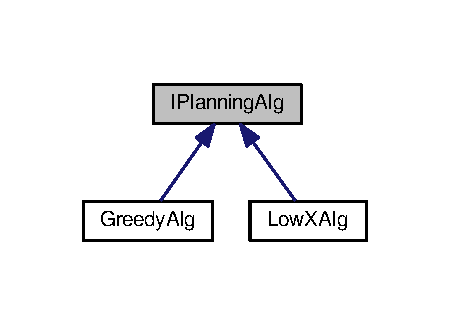
\includegraphics[width=216pt]{classIPlanningAlg__inherit__graph}
\end{center}
\end{figure}
\subsection*{Public Member Functions}
\begin{DoxyCompactItemize}
\item 
virtual void \hyperlink{classIPlanningAlg_abae4e6198042e0acf9abec46e624cd14}{create\+Plan} (\hyperlink{classPoint}{Point} robot\+Location)=0
\begin{DoxyCompactList}\small\item\em Virtual function for creating Plan. \end{DoxyCompactList}\item 
virtual void \hyperlink{classIPlanningAlg_a2bda969cf89a041cb9fbbc7574e7b94f}{push} (\hyperlink{classPoint}{Point} debris\+Location)=0
\begin{DoxyCompactList}\small\item\em Virtual function pusing debris into debris vector. \end{DoxyCompactList}\item 
virtual \hyperlink{classPoint}{Point} \hyperlink{classIPlanningAlg_a4f881df301b194754b1b81ddccad1ed4}{pop} (\hyperlink{classPoint}{Point} robot\+Location)=0
\begin{DoxyCompactList}\small\item\em Virtual function reading and removing top element of debris vector. \end{DoxyCompactList}\end{DoxyCompactItemize}


\subsection{Member Function Documentation}
\index{I\+Planning\+Alg@{I\+Planning\+Alg}!create\+Plan@{create\+Plan}}
\index{create\+Plan@{create\+Plan}!I\+Planning\+Alg@{I\+Planning\+Alg}}
\subsubsection[{\texorpdfstring{create\+Plan(\+Point robot\+Location)=0}{createPlan(Point robotLocation)=0}}]{\setlength{\rightskip}{0pt plus 5cm}virtual void I\+Planning\+Alg\+::create\+Plan (
\begin{DoxyParamCaption}
\item[{{\bf Point}}]{robot\+Location}
\end{DoxyParamCaption}
)\hspace{0.3cm}{\ttfamily [pure virtual]}}\hypertarget{classIPlanningAlg_abae4e6198042e0acf9abec46e624cd14}{}\label{classIPlanningAlg_abae4e6198042e0acf9abec46e624cd14}


Virtual function for creating Plan. 


\begin{DoxyParams}{Parameters}
{\em Robot\textquotesingle{}s} & (x,y) location \\
\hline
\end{DoxyParams}
\begin{DoxyReturn}{Returns}
None 
\end{DoxyReturn}


Implemented in \hyperlink{classLowXAlg_a570c9f04bf3b37b38619e6e6c6f31591}{Low\+X\+Alg}, and \hyperlink{classGreedyAlg_a5048e07294c60d726fdd7c82f0647dc6}{Greedy\+Alg}.

\index{I\+Planning\+Alg@{I\+Planning\+Alg}!pop@{pop}}
\index{pop@{pop}!I\+Planning\+Alg@{I\+Planning\+Alg}}
\subsubsection[{\texorpdfstring{pop(\+Point robot\+Location)=0}{pop(Point robotLocation)=0}}]{\setlength{\rightskip}{0pt plus 5cm}virtual {\bf Point} I\+Planning\+Alg\+::pop (
\begin{DoxyParamCaption}
\item[{{\bf Point}}]{robot\+Location}
\end{DoxyParamCaption}
)\hspace{0.3cm}{\ttfamily [pure virtual]}}\hypertarget{classIPlanningAlg_a4f881df301b194754b1b81ddccad1ed4}{}\label{classIPlanningAlg_a4f881df301b194754b1b81ddccad1ed4}


Virtual function reading and removing top element of debris vector. 


\begin{DoxyParams}{Parameters}
{\em Robot\textquotesingle{}s} & (x,y) location \\
\hline
\end{DoxyParams}
\begin{DoxyReturn}{Returns}
None 
\end{DoxyReturn}


Implemented in \hyperlink{classLowXAlg_a3f331a3ec443d39e07378a7412c2d2f0}{Low\+X\+Alg}, and \hyperlink{classGreedyAlg_a72f7ee716b3c2010070e0f729780d203}{Greedy\+Alg}.

\index{I\+Planning\+Alg@{I\+Planning\+Alg}!push@{push}}
\index{push@{push}!I\+Planning\+Alg@{I\+Planning\+Alg}}
\subsubsection[{\texorpdfstring{push(\+Point debris\+Location)=0}{push(Point debrisLocation)=0}}]{\setlength{\rightskip}{0pt plus 5cm}virtual void I\+Planning\+Alg\+::push (
\begin{DoxyParamCaption}
\item[{{\bf Point}}]{debris\+Location}
\end{DoxyParamCaption}
)\hspace{0.3cm}{\ttfamily [pure virtual]}}\hypertarget{classIPlanningAlg_a2bda969cf89a041cb9fbbc7574e7b94f}{}\label{classIPlanningAlg_a2bda969cf89a041cb9fbbc7574e7b94f}


Virtual function pusing debris into debris vector. 


\begin{DoxyParams}{Parameters}
{\em Debris} & current location \\
\hline
\end{DoxyParams}
\begin{DoxyReturn}{Returns}
None 
\end{DoxyReturn}


Implemented in \hyperlink{classLowXAlg_ac7fdd27ebd0d53ac7d6cbac213324645}{Low\+X\+Alg}, and \hyperlink{classGreedyAlg_a4ce065242ae545ec81ea4599c3b5fcdd}{Greedy\+Alg}.



The documentation for this class was generated from the following file\+:\begin{DoxyCompactItemize}
\item 
/home/lydiazoghbi/catkin\+\_\+ws/src/project\+\_\+x\+\_\+ecobot/include/\hyperlink{IPlanningAlg_8hpp}{I\+Planning\+Alg.\+hpp}\end{DoxyCompactItemize}

\hypertarget{classLowXAlg}{}\section{Low\+X\+Alg Class Reference}
\label{classLowXAlg}\index{Low\+X\+Alg@{Low\+X\+Alg}}


{\ttfamily \#include $<$Low\+X\+Alg.\+hpp$>$}



Inheritance diagram for Low\+X\+Alg\+:
\nopagebreak
\begin{figure}[H]
\begin{center}
\leavevmode
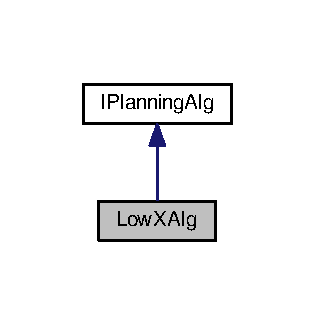
\includegraphics[width=151pt]{classLowXAlg__inherit__graph}
\end{center}
\end{figure}


Collaboration diagram for Low\+X\+Alg\+:
\nopagebreak
\begin{figure}[H]
\begin{center}
\leavevmode
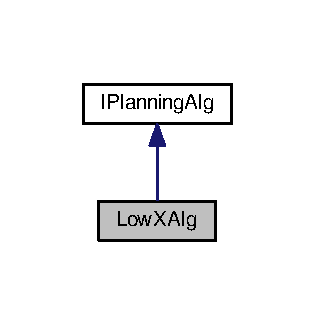
\includegraphics[width=151pt]{classLowXAlg__coll__graph}
\end{center}
\end{figure}
\subsection*{Public Member Functions}
\begin{DoxyCompactItemize}
\item 
\hyperlink{classLowXAlg_a63964d352845bacbdecbccac3c753b17}{$\sim$\+Low\+X\+Alg} ()
\begin{DoxyCompactList}\small\item\em Destructor for the \hyperlink{classLowXAlg}{Low\+X\+Alg} class. \end{DoxyCompactList}\item 
void \hyperlink{classLowXAlg_a570c9f04bf3b37b38619e6e6c6f31591}{create\+Plan} (\hyperlink{classPoint}{Point} robot\+Location)
\begin{DoxyCompactList}\small\item\em Plan creation for how to pick up the debris. \end{DoxyCompactList}\item 
void \hyperlink{classLowXAlg_ac7fdd27ebd0d53ac7d6cbac213324645}{push} (\hyperlink{classPoint}{Point} debris\+Location)
\begin{DoxyCompactList}\small\item\em Function for adding the debris into a debris vector. \end{DoxyCompactList}\item 
\hyperlink{classPoint}{Point} \hyperlink{classLowXAlg_a3f331a3ec443d39e07378a7412c2d2f0}{pop} (\hyperlink{classPoint}{Point} robot\+Location)
\begin{DoxyCompactList}\small\item\em Function for extracting the debris on the top of the vector. \end{DoxyCompactList}\end{DoxyCompactItemize}


\subsection{Constructor \& Destructor Documentation}
\index{Low\+X\+Alg@{Low\+X\+Alg}!````~Low\+X\+Alg@{$\sim$\+Low\+X\+Alg}}
\index{````~Low\+X\+Alg@{$\sim$\+Low\+X\+Alg}!Low\+X\+Alg@{Low\+X\+Alg}}
\subsubsection[{\texorpdfstring{$\sim$\+Low\+X\+Alg()}{~LowXAlg()}}]{\setlength{\rightskip}{0pt plus 5cm}Low\+X\+Alg\+::$\sim$\+Low\+X\+Alg (
\begin{DoxyParamCaption}
{}
\end{DoxyParamCaption}
)}\hypertarget{classLowXAlg_a63964d352845bacbdecbccac3c753b17}{}\label{classLowXAlg_a63964d352845bacbdecbccac3c753b17}


Destructor for the \hyperlink{classLowXAlg}{Low\+X\+Alg} class. 


\begin{DoxyParams}{Parameters}
{\em None} & \\
\hline
\end{DoxyParams}
\begin{DoxyReturn}{Returns}
None 
\end{DoxyReturn}


\subsection{Member Function Documentation}
\index{Low\+X\+Alg@{Low\+X\+Alg}!create\+Plan@{create\+Plan}}
\index{create\+Plan@{create\+Plan}!Low\+X\+Alg@{Low\+X\+Alg}}
\subsubsection[{\texorpdfstring{create\+Plan(\+Point robot\+Location)}{createPlan(Point robotLocation)}}]{\setlength{\rightskip}{0pt plus 5cm}void Low\+X\+Alg\+::create\+Plan (
\begin{DoxyParamCaption}
\item[{{\bf Point}}]{robot\+Location}
\end{DoxyParamCaption}
)\hspace{0.3cm}{\ttfamily [virtual]}}\hypertarget{classLowXAlg_a570c9f04bf3b37b38619e6e6c6f31591}{}\label{classLowXAlg_a570c9f04bf3b37b38619e6e6c6f31591}


Plan creation for how to pick up the debris. 


\begin{DoxyParams}{Parameters}
{\em Robot\textquotesingle{}s} & current (x,y) location \\
\hline
\end{DoxyParams}
\begin{DoxyReturn}{Returns}
None 
\end{DoxyReturn}


Implements \hyperlink{classIPlanningAlg_abae4e6198042e0acf9abec46e624cd14}{I\+Planning\+Alg}.

\index{Low\+X\+Alg@{Low\+X\+Alg}!pop@{pop}}
\index{pop@{pop}!Low\+X\+Alg@{Low\+X\+Alg}}
\subsubsection[{\texorpdfstring{pop(\+Point robot\+Location)}{pop(Point robotLocation)}}]{\setlength{\rightskip}{0pt plus 5cm}{\bf Point} Low\+X\+Alg\+::pop (
\begin{DoxyParamCaption}
\item[{{\bf Point}}]{robot\+Location}
\end{DoxyParamCaption}
)\hspace{0.3cm}{\ttfamily [virtual]}}\hypertarget{classLowXAlg_a3f331a3ec443d39e07378a7412c2d2f0}{}\label{classLowXAlg_a3f331a3ec443d39e07378a7412c2d2f0}


Function for extracting the debris on the top of the vector. 


\begin{DoxyParams}{Parameters}
{\em Robot\textquotesingle{}s} & current (x,y) location \\
\hline
\end{DoxyParams}
\begin{DoxyReturn}{Returns}
Position of debris 
\end{DoxyReturn}


Implements \hyperlink{classIPlanningAlg_a4f881df301b194754b1b81ddccad1ed4}{I\+Planning\+Alg}.

\index{Low\+X\+Alg@{Low\+X\+Alg}!push@{push}}
\index{push@{push}!Low\+X\+Alg@{Low\+X\+Alg}}
\subsubsection[{\texorpdfstring{push(\+Point debris\+Location)}{push(Point debrisLocation)}}]{\setlength{\rightskip}{0pt plus 5cm}void Low\+X\+Alg\+::push (
\begin{DoxyParamCaption}
\item[{{\bf Point}}]{debris\+Location}
\end{DoxyParamCaption}
)\hspace{0.3cm}{\ttfamily [virtual]}}\hypertarget{classLowXAlg_ac7fdd27ebd0d53ac7d6cbac213324645}{}\label{classLowXAlg_ac7fdd27ebd0d53ac7d6cbac213324645}


Function for adding the debris into a debris vector. 


\begin{DoxyParams}{Parameters}
{\em Observed} & debris location \\
\hline
\end{DoxyParams}
\begin{DoxyReturn}{Returns}
None 
\end{DoxyReturn}


Implements \hyperlink{classIPlanningAlg_a2bda969cf89a041cb9fbbc7574e7b94f}{I\+Planning\+Alg}.



The documentation for this class was generated from the following file\+:\begin{DoxyCompactItemize}
\item 
/home/lydiazoghbi/catkin\+\_\+ws/src/project\+\_\+x\+\_\+ecobot/include/\hyperlink{LowXAlg_8hpp}{Low\+X\+Alg.\+hpp}\end{DoxyCompactItemize}

\hypertarget{classPoint}{}\section{Point Class Reference}
\label{classPoint}\index{Point@{Point}}


{\ttfamily \#include $<$Point.\+hpp$>$}

\subsection*{Public Member Functions}
\begin{DoxyCompactItemize}
\item 
\hyperlink{classPoint_af85be1aa9a54381d93458ada09289e07}{Point} (double startX=0, double startY=0)
\begin{DoxyCompactList}\small\item\em Constructor for \hyperlink{classPoint}{Point} class. \end{DoxyCompactList}\item 
double \hyperlink{classPoint_a8de35a6098cdd7267b4167776da83da6}{getX} ()
\begin{DoxyCompactList}\small\item\em Function to obtain x value. \end{DoxyCompactList}\item 
double \hyperlink{classPoint_aa278c8bcb8aeb4101023a4baf473b547}{getY} ()
\begin{DoxyCompactList}\small\item\em Function to obtain y value. \end{DoxyCompactList}\end{DoxyCompactItemize}


\subsection{Constructor \& Destructor Documentation}
\index{Point@{Point}!Point@{Point}}
\index{Point@{Point}!Point@{Point}}
\subsubsection[{\texorpdfstring{Point(double start\+X=0, double start\+Y=0)}{Point(double startX=0, double startY=0)}}]{\setlength{\rightskip}{0pt plus 5cm}Point\+::\+Point (
\begin{DoxyParamCaption}
\item[{double}]{startX = {\ttfamily 0}, }
\item[{double}]{startY = {\ttfamily 0}}
\end{DoxyParamCaption}
)\hspace{0.3cm}{\ttfamily [explicit]}}\hypertarget{classPoint_af85be1aa9a54381d93458ada09289e07}{}\label{classPoint_af85be1aa9a54381d93458ada09289e07}


Constructor for \hyperlink{classPoint}{Point} class. 


\begin{DoxyParams}{Parameters}
{\em An} & initial point x \\
\hline
{\em An} & initial point y \\
\hline
\end{DoxyParams}
\begin{DoxyReturn}{Returns}
None 
\end{DoxyReturn}


\subsection{Member Function Documentation}
\index{Point@{Point}!getX@{getX}}
\index{getX@{getX}!Point@{Point}}
\subsubsection[{\texorpdfstring{get\+X()}{getX()}}]{\setlength{\rightskip}{0pt plus 5cm}double Point\+::getX (
\begin{DoxyParamCaption}
{}
\end{DoxyParamCaption}
)}\hypertarget{classPoint_a8de35a6098cdd7267b4167776da83da6}{}\label{classPoint_a8de35a6098cdd7267b4167776da83da6}


Function to obtain x value. 


\begin{DoxyParams}{Parameters}
{\em None} & \\
\hline
\end{DoxyParams}
\begin{DoxyReturn}{Returns}
The x value that was stored from the constructor 
\end{DoxyReturn}
\index{Point@{Point}!getY@{getY}}
\index{getY@{getY}!Point@{Point}}
\subsubsection[{\texorpdfstring{get\+Y()}{getY()}}]{\setlength{\rightskip}{0pt plus 5cm}double Point\+::getY (
\begin{DoxyParamCaption}
{}
\end{DoxyParamCaption}
)}\hypertarget{classPoint_aa278c8bcb8aeb4101023a4baf473b547}{}\label{classPoint_aa278c8bcb8aeb4101023a4baf473b547}


Function to obtain y value. 


\begin{DoxyParams}{Parameters}
{\em None} & \\
\hline
\end{DoxyParams}
\begin{DoxyReturn}{Returns}
The y value that was stored from the constructor 
\end{DoxyReturn}


The documentation for this class was generated from the following file\+:\begin{DoxyCompactItemize}
\item 
/home/lydiazoghbi/catkin\+\_\+ws/src/project\+\_\+x\+\_\+ecobot/include/\hyperlink{Point_8hpp}{Point.\+hpp}\end{DoxyCompactItemize}

\hypertarget{classStateMachine}{}\section{State\+Machine Class Reference}
\label{classStateMachine}\index{State\+Machine@{State\+Machine}}


{\ttfamily \#include $<$State\+Machine.\+hpp$>$}

\subsection*{Public Types}
\begin{DoxyCompactItemize}
\item 
enum \hyperlink{classStateMachine_a08a90356de9073dd0ee4d56b74d2e823}{State} \+: int \{ \\*
\hyperlink{classStateMachine_a08a90356de9073dd0ee4d56b74d2e823a016d5abef569ab6b71056250fe22521d}{placeholder\+State} = -\/1, 
\hyperlink{classStateMachine_a08a90356de9073dd0ee4d56b74d2e823aab795cc7ada954f7046748f8e88917a8}{initial\+Scan\+For\+Debris} = 0, 
\hyperlink{classStateMachine_a08a90356de9073dd0ee4d56b74d2e823a9b5e93ae092b0bac501ec9e841cc0fd5}{approach\+Debris} = 1, 
\hyperlink{classStateMachine_a08a90356de9073dd0ee4d56b74d2e823a389652ffeb926cc37fd7503492a63d7b}{turn\+Towards\+Bin} = 2, 
\\*
\hyperlink{classStateMachine_a08a90356de9073dd0ee4d56b74d2e823a25a1d720a624c4c11aa7c972337a1d39}{drive\+Towards\+Bin} = 3, 
\hyperlink{classStateMachine_a08a90356de9073dd0ee4d56b74d2e823a0ed933bb47dc0771235542bda24b609e}{turn\+Towards\+Target} = 4, 
\hyperlink{classStateMachine_a08a90356de9073dd0ee4d56b74d2e823ad30b1a10a1847f4f5d533d06c46a269f}{done} = 5
 \}\begin{DoxyCompactList}\small\item\em Enum state elements. \end{DoxyCompactList}
\end{DoxyCompactItemize}
\subsection*{Public Member Functions}
\begin{DoxyCompactItemize}
\item 
\hyperlink{classStateMachine_a6e640066c98dd3acd70e63d8a2c2282b}{State\+Machine} (bool start\+Immediately=false, bool use\+Low\+X\+Algorithm=false)
\begin{DoxyCompactList}\small\item\em Constructor for \hyperlink{classStateMachine}{State\+Machine}. \end{DoxyCompactList}\item 
void \hyperlink{classStateMachine_aab9afe1c41b8c88e9fe2e2c4be227bfb}{image\+R\+G\+B\+Callback} (const sensor\+\_\+msgs\+::\+Image\+Const\+Ptr \&message)
\begin{DoxyCompactList}\small\item\em Callback function to obtain the images. \end{DoxyCompactList}\item 
void \hyperlink{classStateMachine_a64cd46adabf0963ea057535ab8bba849}{odometry\+Callback} (const nav\+\_\+msgs\+::\+Odometry\+::\+Const\+Ptr \&message)
\begin{DoxyCompactList}\small\item\em Callback function to obtain the odometry. \end{DoxyCompactList}\item 
void \hyperlink{classStateMachine_a1502417471ac1ab34c2e9e3a34bf8f4c}{depth\+Callback} (const sensor\+\_\+msgs\+::\+Image\+Const\+Ptr \&depth\+Message)
\begin{DoxyCompactList}\small\item\em Callback function to obtain depth information from the images. \end{DoxyCompactList}\item 
double \hyperlink{classStateMachine_ae70aff20d71caa15c22b5ae5de8f76af}{read\+Depth\+Data} (unsigned int height\+Pos, unsigned int width\+Pos, sensor\+\_\+msgs\+::\+Image\+Const\+Ptr depth\+Image)
\begin{DoxyCompactList}\small\item\em Function for obtaining depth information at certain image pixel position. \end{DoxyCompactList}\item 
bool \hyperlink{classStateMachine_a68b85b66b901ee8fbd9c7be93487f28f}{pickup\+Debris} (\hyperlink{classStateMachine_a08a90356de9073dd0ee4d56b74d2e823}{State} end\+State=\hyperlink{classStateMachine_a08a90356de9073dd0ee4d56b74d2e823a016d5abef569ab6b71056250fe22521d}{placeholder\+State}, \hyperlink{classStateMachine_a08a90356de9073dd0ee4d56b74d2e823}{State} start\+State=\hyperlink{classStateMachine_a08a90356de9073dd0ee4d56b74d2e823aab795cc7ada954f7046748f8e88917a8}{initial\+Scan\+For\+Debris}, double registered\+Depth=0.\+0, double fake\+Depth=-\/1.\+0)
\begin{DoxyCompactList}\small\item\em Function for running the main ros loop. \end{DoxyCompactList}\item 
double \hyperlink{classStateMachine_a4bdbecd6cf56fb8fff20c7e0232dd33b}{get\+Raw\+Depth} ()
\begin{DoxyCompactList}\small\item\em Getter function for taking depth as input. \end{DoxyCompactList}\item 
int \hyperlink{classStateMachine_ae386ede5033e27c114e88bdd830a6ff2}{get\+State} ()
\begin{DoxyCompactList}\small\item\em Getter function for reading robot\textquotesingle{}s state. \end{DoxyCompactList}\item 
cv\+::\+Mat \hyperlink{classStateMachine_a3f545ec499f6136057d9ecf44663d3a3}{get\+Image} ()
\begin{DoxyCompactList}\small\item\em Getter function for taking in the image. \end{DoxyCompactList}\item 
double \hyperlink{classStateMachine_a99887795ff6b06f6002779f72928d330}{get\+Robot\+X\+Pos} ()
\begin{DoxyCompactList}\small\item\em Getter function for obtaining robot\textquotesingle{}s x position. \end{DoxyCompactList}\item 
double \hyperlink{classStateMachine_a4bc3adc3985724e42ab8509457b59ad0}{get\+Robot\+Y\+Pos} ()
\begin{DoxyCompactList}\small\item\em Getter function for obtaining robot\textquotesingle{}s y position. \end{DoxyCompactList}\item 
double \hyperlink{classStateMachine_ab9c545cbbf1ccae25a4c68e4d1323751}{get\+Robot\+Yaw} ()
\begin{DoxyCompactList}\small\item\em Getter function for obtaining robot\textquotesingle{}s yaw angle (orientation) \end{DoxyCompactList}\item 
double \hyperlink{classStateMachine_a82c53e5941ba7b2b96eff859bbf9d754}{get\+Depth} ()
\begin{DoxyCompactList}\small\item\em Getter function for obtaining depth read from camera. \end{DoxyCompactList}\item 
double \hyperlink{classStateMachine_ae489fcd0f460527700e3e4de549b5bf6}{verify\+Angle} (double raw\+Angle)
\begin{DoxyCompactList}\small\item\em Function for casting angle between 0 and 2\+PI. \end{DoxyCompactList}\item 
geometry\+\_\+msgs\+::\+Twist \hyperlink{classStateMachine_a78b255b75372d19a0f89634b268fe5da}{stop} (geometry\+\_\+msgs\+::\+Twist velocity)
\begin{DoxyCompactList}\small\item\em Function to stop robot\textquotesingle{}s motion. \end{DoxyCompactList}\item 
geometry\+\_\+msgs\+::\+Twist \hyperlink{classStateMachine_a6718533fefd33ee2b73f4ede6aa53e22}{move\+Straight} (geometry\+\_\+msgs\+::\+Twist velocity)
\begin{DoxyCompactList}\small\item\em Function to move the robot forward (straight) \end{DoxyCompactList}\item 
geometry\+\_\+msgs\+::\+Twist \hyperlink{classStateMachine_a1c3bfb5713c29ff24f440c2105308769}{turn\+Right} (geometry\+\_\+msgs\+::\+Twist velocity)
\begin{DoxyCompactList}\small\item\em Function to turn the robot to the right. \end{DoxyCompactList}\item 
geometry\+\_\+msgs\+::\+Twist \hyperlink{classStateMachine_ac1e4e9e429332b41f7c35300302f0c75}{turn\+Left} (geometry\+\_\+msgs\+::\+Twist velocity)
\begin{DoxyCompactList}\small\item\em Function to turn the robot to the left. \end{DoxyCompactList}\end{DoxyCompactItemize}


\subsection{Member Enumeration Documentation}
\index{State\+Machine@{State\+Machine}!State@{State}}
\index{State@{State}!State\+Machine@{State\+Machine}}
\subsubsection[{\texorpdfstring{State}{State}}]{\setlength{\rightskip}{0pt plus 5cm}enum {\bf State\+Machine\+::\+State} \+: int}\hypertarget{classStateMachine_a08a90356de9073dd0ee4d56b74d2e823}{}\label{classStateMachine_a08a90356de9073dd0ee4d56b74d2e823}


Enum state elements. 


\begin{DoxyParams}{Parameters}
{\em None} & \\
\hline
\end{DoxyParams}
\begin{DoxyReturn}{Returns}
Enum 
\end{DoxyReturn}
\begin{Desc}
\item[Enumerator]\par
\begin{description}
\index{placeholder\+State@{placeholder\+State}!State\+Machine@{State\+Machine}}\index{State\+Machine@{State\+Machine}!placeholder\+State@{placeholder\+State}}\item[{\em 
placeholder\+State\hypertarget{classStateMachine_a08a90356de9073dd0ee4d56b74d2e823a016d5abef569ab6b71056250fe22521d}{}\label{classStateMachine_a08a90356de9073dd0ee4d56b74d2e823a016d5abef569ab6b71056250fe22521d}
}]\index{initial\+Scan\+For\+Debris@{initial\+Scan\+For\+Debris}!State\+Machine@{State\+Machine}}\index{State\+Machine@{State\+Machine}!initial\+Scan\+For\+Debris@{initial\+Scan\+For\+Debris}}\item[{\em 
initial\+Scan\+For\+Debris\hypertarget{classStateMachine_a08a90356de9073dd0ee4d56b74d2e823aab795cc7ada954f7046748f8e88917a8}{}\label{classStateMachine_a08a90356de9073dd0ee4d56b74d2e823aab795cc7ada954f7046748f8e88917a8}
}]\index{approach\+Debris@{approach\+Debris}!State\+Machine@{State\+Machine}}\index{State\+Machine@{State\+Machine}!approach\+Debris@{approach\+Debris}}\item[{\em 
approach\+Debris\hypertarget{classStateMachine_a08a90356de9073dd0ee4d56b74d2e823a9b5e93ae092b0bac501ec9e841cc0fd5}{}\label{classStateMachine_a08a90356de9073dd0ee4d56b74d2e823a9b5e93ae092b0bac501ec9e841cc0fd5}
}]\index{turn\+Towards\+Bin@{turn\+Towards\+Bin}!State\+Machine@{State\+Machine}}\index{State\+Machine@{State\+Machine}!turn\+Towards\+Bin@{turn\+Towards\+Bin}}\item[{\em 
turn\+Towards\+Bin\hypertarget{classStateMachine_a08a90356de9073dd0ee4d56b74d2e823a389652ffeb926cc37fd7503492a63d7b}{}\label{classStateMachine_a08a90356de9073dd0ee4d56b74d2e823a389652ffeb926cc37fd7503492a63d7b}
}]\index{drive\+Towards\+Bin@{drive\+Towards\+Bin}!State\+Machine@{State\+Machine}}\index{State\+Machine@{State\+Machine}!drive\+Towards\+Bin@{drive\+Towards\+Bin}}\item[{\em 
drive\+Towards\+Bin\hypertarget{classStateMachine_a08a90356de9073dd0ee4d56b74d2e823a25a1d720a624c4c11aa7c972337a1d39}{}\label{classStateMachine_a08a90356de9073dd0ee4d56b74d2e823a25a1d720a624c4c11aa7c972337a1d39}
}]\index{turn\+Towards\+Target@{turn\+Towards\+Target}!State\+Machine@{State\+Machine}}\index{State\+Machine@{State\+Machine}!turn\+Towards\+Target@{turn\+Towards\+Target}}\item[{\em 
turn\+Towards\+Target\hypertarget{classStateMachine_a08a90356de9073dd0ee4d56b74d2e823a0ed933bb47dc0771235542bda24b609e}{}\label{classStateMachine_a08a90356de9073dd0ee4d56b74d2e823a0ed933bb47dc0771235542bda24b609e}
}]\index{done@{done}!State\+Machine@{State\+Machine}}\index{State\+Machine@{State\+Machine}!done@{done}}\item[{\em 
done\hypertarget{classStateMachine_a08a90356de9073dd0ee4d56b74d2e823ad30b1a10a1847f4f5d533d06c46a269f}{}\label{classStateMachine_a08a90356de9073dd0ee4d56b74d2e823ad30b1a10a1847f4f5d533d06c46a269f}
}]\end{description}
\end{Desc}


\subsection{Constructor \& Destructor Documentation}
\index{State\+Machine@{State\+Machine}!State\+Machine@{State\+Machine}}
\index{State\+Machine@{State\+Machine}!State\+Machine@{State\+Machine}}
\subsubsection[{\texorpdfstring{State\+Machine(bool start\+Immediately=false, bool use\+Low\+X\+Algorithm=false)}{StateMachine(bool startImmediately=false, bool useLowXAlgorithm=false)}}]{\setlength{\rightskip}{0pt plus 5cm}State\+Machine\+::\+State\+Machine (
\begin{DoxyParamCaption}
\item[{bool}]{start\+Immediately = {\ttfamily false}, }
\item[{bool}]{use\+Low\+X\+Algorithm = {\ttfamily false}}
\end{DoxyParamCaption}
)\hspace{0.3cm}{\ttfamily [explicit]}}\hypertarget{classStateMachine_a6e640066c98dd3acd70e63d8a2c2282b}{}\label{classStateMachine_a6e640066c98dd3acd70e63d8a2c2282b}


Constructor for \hyperlink{classStateMachine}{State\+Machine}. 


\begin{DoxyParams}{Parameters}
{\em Boolean} & for starting immediately or waiting \\
\hline
{\em Boolean} & for choosing which algorithm to use \\
\hline
\end{DoxyParams}
\begin{DoxyReturn}{Returns}
None 
\end{DoxyReturn}


\subsection{Member Function Documentation}
\index{State\+Machine@{State\+Machine}!depth\+Callback@{depth\+Callback}}
\index{depth\+Callback@{depth\+Callback}!State\+Machine@{State\+Machine}}
\subsubsection[{\texorpdfstring{depth\+Callback(const sensor\+\_\+msgs\+::\+Image\+Const\+Ptr \&depth\+Message)}{depthCallback(const sensor_msgs::ImageConstPtr &depthMessage)}}]{\setlength{\rightskip}{0pt plus 5cm}void State\+Machine\+::depth\+Callback (
\begin{DoxyParamCaption}
\item[{const sensor\+\_\+msgs\+::\+Image\+Const\+Ptr \&}]{depth\+Message}
\end{DoxyParamCaption}
)}\hypertarget{classStateMachine_a1502417471ac1ab34c2e9e3a34bf8f4c}{}\label{classStateMachine_a1502417471ac1ab34c2e9e3a34bf8f4c}


Callback function to obtain depth information from the images. 


\begin{DoxyParams}{Parameters}
{\em A} & ros message which is the depth reading \\
\hline
\end{DoxyParams}
\begin{DoxyReturn}{Returns}
Depth of selected point in image, nothing explicit 
\end{DoxyReturn}
\index{State\+Machine@{State\+Machine}!get\+Depth@{get\+Depth}}
\index{get\+Depth@{get\+Depth}!State\+Machine@{State\+Machine}}
\subsubsection[{\texorpdfstring{get\+Depth()}{getDepth()}}]{\setlength{\rightskip}{0pt plus 5cm}double State\+Machine\+::get\+Depth (
\begin{DoxyParamCaption}
{}
\end{DoxyParamCaption}
)}\hypertarget{classStateMachine_a82c53e5941ba7b2b96eff859bbf9d754}{}\label{classStateMachine_a82c53e5941ba7b2b96eff859bbf9d754}


Getter function for obtaining depth read from camera. 


\begin{DoxyParams}{Parameters}
{\em None} & \\
\hline
\end{DoxyParams}
\begin{DoxyReturn}{Returns}
Double depth value 
\end{DoxyReturn}
\index{State\+Machine@{State\+Machine}!get\+Image@{get\+Image}}
\index{get\+Image@{get\+Image}!State\+Machine@{State\+Machine}}
\subsubsection[{\texorpdfstring{get\+Image()}{getImage()}}]{\setlength{\rightskip}{0pt plus 5cm}cv\+::\+Mat State\+Machine\+::get\+Image (
\begin{DoxyParamCaption}
{}
\end{DoxyParamCaption}
)}\hypertarget{classStateMachine_a3f545ec499f6136057d9ecf44663d3a3}{}\label{classStateMachine_a3f545ec499f6136057d9ecf44663d3a3}


Getter function for taking in the image. 


\begin{DoxyParams}{Parameters}
{\em None} & \\
\hline
\end{DoxyParams}
\begin{DoxyReturn}{Returns}
Returned image 
\end{DoxyReturn}
\index{State\+Machine@{State\+Machine}!get\+Raw\+Depth@{get\+Raw\+Depth}}
\index{get\+Raw\+Depth@{get\+Raw\+Depth}!State\+Machine@{State\+Machine}}
\subsubsection[{\texorpdfstring{get\+Raw\+Depth()}{getRawDepth()}}]{\setlength{\rightskip}{0pt plus 5cm}double State\+Machine\+::get\+Raw\+Depth (
\begin{DoxyParamCaption}
{}
\end{DoxyParamCaption}
)}\hypertarget{classStateMachine_a4bdbecd6cf56fb8fff20c7e0232dd33b}{}\label{classStateMachine_a4bdbecd6cf56fb8fff20c7e0232dd33b}


Getter function for taking depth as input. 


\begin{DoxyParams}{Parameters}
{\em None} & \\
\hline
\end{DoxyParams}
\begin{DoxyReturn}{Returns}
Double depth 
\end{DoxyReturn}
\index{State\+Machine@{State\+Machine}!get\+Robot\+X\+Pos@{get\+Robot\+X\+Pos}}
\index{get\+Robot\+X\+Pos@{get\+Robot\+X\+Pos}!State\+Machine@{State\+Machine}}
\subsubsection[{\texorpdfstring{get\+Robot\+X\+Pos()}{getRobotXPos()}}]{\setlength{\rightskip}{0pt plus 5cm}double State\+Machine\+::get\+Robot\+X\+Pos (
\begin{DoxyParamCaption}
{}
\end{DoxyParamCaption}
)}\hypertarget{classStateMachine_a99887795ff6b06f6002779f72928d330}{}\label{classStateMachine_a99887795ff6b06f6002779f72928d330}


Getter function for obtaining robot\textquotesingle{}s x position. 


\begin{DoxyParams}{Parameters}
{\em None} & \\
\hline
\end{DoxyParams}
\begin{DoxyReturn}{Returns}
Double x position 
\end{DoxyReturn}
\index{State\+Machine@{State\+Machine}!get\+Robot\+Yaw@{get\+Robot\+Yaw}}
\index{get\+Robot\+Yaw@{get\+Robot\+Yaw}!State\+Machine@{State\+Machine}}
\subsubsection[{\texorpdfstring{get\+Robot\+Yaw()}{getRobotYaw()}}]{\setlength{\rightskip}{0pt plus 5cm}double State\+Machine\+::get\+Robot\+Yaw (
\begin{DoxyParamCaption}
{}
\end{DoxyParamCaption}
)}\hypertarget{classStateMachine_ab9c545cbbf1ccae25a4c68e4d1323751}{}\label{classStateMachine_ab9c545cbbf1ccae25a4c68e4d1323751}


Getter function for obtaining robot\textquotesingle{}s yaw angle (orientation) 


\begin{DoxyParams}{Parameters}
{\em None} & \\
\hline
\end{DoxyParams}
\begin{DoxyReturn}{Returns}
Orientattion 
\end{DoxyReturn}
\index{State\+Machine@{State\+Machine}!get\+Robot\+Y\+Pos@{get\+Robot\+Y\+Pos}}
\index{get\+Robot\+Y\+Pos@{get\+Robot\+Y\+Pos}!State\+Machine@{State\+Machine}}
\subsubsection[{\texorpdfstring{get\+Robot\+Y\+Pos()}{getRobotYPos()}}]{\setlength{\rightskip}{0pt plus 5cm}double State\+Machine\+::get\+Robot\+Y\+Pos (
\begin{DoxyParamCaption}
{}
\end{DoxyParamCaption}
)}\hypertarget{classStateMachine_a4bc3adc3985724e42ab8509457b59ad0}{}\label{classStateMachine_a4bc3adc3985724e42ab8509457b59ad0}


Getter function for obtaining robot\textquotesingle{}s y position. 


\begin{DoxyParams}{Parameters}
{\em None} & \\
\hline
\end{DoxyParams}
\begin{DoxyReturn}{Returns}
Double y position 
\end{DoxyReturn}
\index{State\+Machine@{State\+Machine}!get\+State@{get\+State}}
\index{get\+State@{get\+State}!State\+Machine@{State\+Machine}}
\subsubsection[{\texorpdfstring{get\+State()}{getState()}}]{\setlength{\rightskip}{0pt plus 5cm}int State\+Machine\+::get\+State (
\begin{DoxyParamCaption}
{}
\end{DoxyParamCaption}
)}\hypertarget{classStateMachine_ae386ede5033e27c114e88bdd830a6ff2}{}\label{classStateMachine_ae386ede5033e27c114e88bdd830a6ff2}


Getter function for reading robot\textquotesingle{}s state. 


\begin{DoxyParams}{Parameters}
{\em None} & \\
\hline
\end{DoxyParams}
\begin{DoxyReturn}{Returns}
Integer robot\textquotesingle{}s state 
\end{DoxyReturn}
\index{State\+Machine@{State\+Machine}!image\+R\+G\+B\+Callback@{image\+R\+G\+B\+Callback}}
\index{image\+R\+G\+B\+Callback@{image\+R\+G\+B\+Callback}!State\+Machine@{State\+Machine}}
\subsubsection[{\texorpdfstring{image\+R\+G\+B\+Callback(const sensor\+\_\+msgs\+::\+Image\+Const\+Ptr \&message)}{imageRGBCallback(const sensor_msgs::ImageConstPtr &message)}}]{\setlength{\rightskip}{0pt plus 5cm}void State\+Machine\+::image\+R\+G\+B\+Callback (
\begin{DoxyParamCaption}
\item[{const sensor\+\_\+msgs\+::\+Image\+Const\+Ptr \&}]{message}
\end{DoxyParamCaption}
)}\hypertarget{classStateMachine_aab9afe1c41b8c88e9fe2e2c4be227bfb}{}\label{classStateMachine_aab9afe1c41b8c88e9fe2e2c4be227bfb}


Callback function to obtain the images. 


\begin{DoxyParams}{Parameters}
{\em A} & ros message which is the R\+GB image \\
\hline
\end{DoxyParams}
\begin{DoxyReturn}{Returns}
An R\+GB image to the subscriber, nothing explicit from function 
\end{DoxyReturn}
\index{State\+Machine@{State\+Machine}!move\+Straight@{move\+Straight}}
\index{move\+Straight@{move\+Straight}!State\+Machine@{State\+Machine}}
\subsubsection[{\texorpdfstring{move\+Straight(geometry\+\_\+msgs\+::\+Twist velocity)}{moveStraight(geometry_msgs::Twist velocity)}}]{\setlength{\rightskip}{0pt plus 5cm}geometry\+\_\+msgs\+::\+Twist State\+Machine\+::move\+Straight (
\begin{DoxyParamCaption}
\item[{geometry\+\_\+msgs\+::\+Twist}]{velocity}
\end{DoxyParamCaption}
)}\hypertarget{classStateMachine_a6718533fefd33ee2b73f4ede6aa53e22}{}\label{classStateMachine_a6718533fefd33ee2b73f4ede6aa53e22}


Function to move the robot forward (straight) 


\begin{DoxyParams}{Parameters}
{\em Geometry} & message velocity \\
\hline
\end{DoxyParams}
\begin{DoxyReturn}{Returns}
Geometry message velocity 
\end{DoxyReturn}
\index{State\+Machine@{State\+Machine}!odometry\+Callback@{odometry\+Callback}}
\index{odometry\+Callback@{odometry\+Callback}!State\+Machine@{State\+Machine}}
\subsubsection[{\texorpdfstring{odometry\+Callback(const nav\+\_\+msgs\+::\+Odometry\+::\+Const\+Ptr \&message)}{odometryCallback(const nav_msgs::Odometry::ConstPtr &message)}}]{\setlength{\rightskip}{0pt plus 5cm}void State\+Machine\+::odometry\+Callback (
\begin{DoxyParamCaption}
\item[{const nav\+\_\+msgs\+::\+Odometry\+::\+Const\+Ptr \&}]{message}
\end{DoxyParamCaption}
)}\hypertarget{classStateMachine_a64cd46adabf0963ea057535ab8bba849}{}\label{classStateMachine_a64cd46adabf0963ea057535ab8bba849}


Callback function to obtain the odometry. 


\begin{DoxyParams}{Parameters}
{\em A} & ros message which is odometry message \\
\hline
\end{DoxyParams}
\begin{DoxyReturn}{Returns}
Turtlebot position and orientation to the subscriber, nothing explicit from function 
\end{DoxyReturn}
\index{State\+Machine@{State\+Machine}!pickup\+Debris@{pickup\+Debris}}
\index{pickup\+Debris@{pickup\+Debris}!State\+Machine@{State\+Machine}}
\subsubsection[{\texorpdfstring{pickup\+Debris(\+State end\+State=placeholder\+State, State start\+State=initial\+Scan\+For\+Debris, double registered\+Depth=0.\+0, double fake\+Depth=-\/1.\+0)}{pickupDebris(State endState=placeholderState, State startState=initialScanForDebris, double registeredDepth=0.0, double fakeDepth=-1.0)}}]{\setlength{\rightskip}{0pt plus 5cm}bool State\+Machine\+::pickup\+Debris (
\begin{DoxyParamCaption}
\item[{{\bf State}}]{end\+State = {\ttfamily {\bf placeholder\+State}}, }
\item[{{\bf State}}]{start\+State = {\ttfamily {\bf initial\+Scan\+For\+Debris}}, }
\item[{double}]{registered\+Depth = {\ttfamily 0.0}, }
\item[{double}]{fake\+Depth = {\ttfamily -\/1.0}}
\end{DoxyParamCaption}
)}\hypertarget{classStateMachine_a68b85b66b901ee8fbd9c7be93487f28f}{}\label{classStateMachine_a68b85b66b901ee8fbd9c7be93487f28f}


Function for running the main ros loop. 


\begin{DoxyParams}{Parameters}
{\em State} & enum for a placeholder\+State \\
\hline
{\em State} & enum for the end state \\
\hline
{\em Depth} & parameter, added for testing purposes \\
\hline
{\em Depth} & parameter, added for testing purposes \\
\hline
\end{DoxyParams}
\begin{DoxyReturn}{Returns}
Boolean true on successful loop termination 
\end{DoxyReturn}
\index{State\+Machine@{State\+Machine}!read\+Depth\+Data@{read\+Depth\+Data}}
\index{read\+Depth\+Data@{read\+Depth\+Data}!State\+Machine@{State\+Machine}}
\subsubsection[{\texorpdfstring{read\+Depth\+Data(unsigned int height\+Pos, unsigned int width\+Pos, sensor\+\_\+msgs\+::\+Image\+Const\+Ptr depth\+Image)}{readDepthData(unsigned int heightPos, unsigned int widthPos, sensor_msgs::ImageConstPtr depthImage)}}]{\setlength{\rightskip}{0pt plus 5cm}double State\+Machine\+::read\+Depth\+Data (
\begin{DoxyParamCaption}
\item[{unsigned int}]{height\+Pos, }
\item[{unsigned int}]{width\+Pos, }
\item[{sensor\+\_\+msgs\+::\+Image\+Const\+Ptr}]{depth\+Image}
\end{DoxyParamCaption}
)}\hypertarget{classStateMachine_ae70aff20d71caa15c22b5ae5de8f76af}{}\label{classStateMachine_ae70aff20d71caa15c22b5ae5de8f76af}


Function for obtaining depth information at certain image pixel position. 


\begin{DoxyParams}{Parameters}
{\em Image} & pixel height \\
\hline
{\em Image} & pixel wdith \\
\hline
{\em Depth} & image from R\+G\+B-\/D camera \\
\hline
\end{DoxyParams}
\begin{DoxyReturn}{Returns}
Depth of specified pixel on image 
\end{DoxyReturn}
\index{State\+Machine@{State\+Machine}!stop@{stop}}
\index{stop@{stop}!State\+Machine@{State\+Machine}}
\subsubsection[{\texorpdfstring{stop(geometry\+\_\+msgs\+::\+Twist velocity)}{stop(geometry_msgs::Twist velocity)}}]{\setlength{\rightskip}{0pt plus 5cm}geometry\+\_\+msgs\+::\+Twist State\+Machine\+::stop (
\begin{DoxyParamCaption}
\item[{geometry\+\_\+msgs\+::\+Twist}]{velocity}
\end{DoxyParamCaption}
)}\hypertarget{classStateMachine_a78b255b75372d19a0f89634b268fe5da}{}\label{classStateMachine_a78b255b75372d19a0f89634b268fe5da}


Function to stop robot\textquotesingle{}s motion. 


\begin{DoxyParams}{Parameters}
{\em Geometry} & message velocity \\
\hline
\end{DoxyParams}
\begin{DoxyReturn}{Returns}
Geometry message velocity 
\end{DoxyReturn}
\index{State\+Machine@{State\+Machine}!turn\+Left@{turn\+Left}}
\index{turn\+Left@{turn\+Left}!State\+Machine@{State\+Machine}}
\subsubsection[{\texorpdfstring{turn\+Left(geometry\+\_\+msgs\+::\+Twist velocity)}{turnLeft(geometry_msgs::Twist velocity)}}]{\setlength{\rightskip}{0pt plus 5cm}geometry\+\_\+msgs\+::\+Twist State\+Machine\+::turn\+Left (
\begin{DoxyParamCaption}
\item[{geometry\+\_\+msgs\+::\+Twist}]{velocity}
\end{DoxyParamCaption}
)}\hypertarget{classStateMachine_ac1e4e9e429332b41f7c35300302f0c75}{}\label{classStateMachine_ac1e4e9e429332b41f7c35300302f0c75}


Function to turn the robot to the left. 


\begin{DoxyParams}{Parameters}
{\em Geometry} & message velocity \\
\hline
\end{DoxyParams}
\begin{DoxyReturn}{Returns}
Geometry message velocity 
\end{DoxyReturn}
\index{State\+Machine@{State\+Machine}!turn\+Right@{turn\+Right}}
\index{turn\+Right@{turn\+Right}!State\+Machine@{State\+Machine}}
\subsubsection[{\texorpdfstring{turn\+Right(geometry\+\_\+msgs\+::\+Twist velocity)}{turnRight(geometry_msgs::Twist velocity)}}]{\setlength{\rightskip}{0pt plus 5cm}geometry\+\_\+msgs\+::\+Twist State\+Machine\+::turn\+Right (
\begin{DoxyParamCaption}
\item[{geometry\+\_\+msgs\+::\+Twist}]{velocity}
\end{DoxyParamCaption}
)}\hypertarget{classStateMachine_a1c3bfb5713c29ff24f440c2105308769}{}\label{classStateMachine_a1c3bfb5713c29ff24f440c2105308769}


Function to turn the robot to the right. 


\begin{DoxyParams}{Parameters}
{\em Geometry} & message velocity \\
\hline
\end{DoxyParams}
\begin{DoxyReturn}{Returns}
Geometry message velocity 
\end{DoxyReturn}
\index{State\+Machine@{State\+Machine}!verify\+Angle@{verify\+Angle}}
\index{verify\+Angle@{verify\+Angle}!State\+Machine@{State\+Machine}}
\subsubsection[{\texorpdfstring{verify\+Angle(double raw\+Angle)}{verifyAngle(double rawAngle)}}]{\setlength{\rightskip}{0pt plus 5cm}double State\+Machine\+::verify\+Angle (
\begin{DoxyParamCaption}
\item[{double}]{raw\+Angle}
\end{DoxyParamCaption}
)}\hypertarget{classStateMachine_ae489fcd0f460527700e3e4de549b5bf6}{}\label{classStateMachine_ae489fcd0f460527700e3e4de549b5bf6}


Function for casting angle between 0 and 2\+PI. 


\begin{DoxyParams}{Parameters}
{\em An} & angle in radians \\
\hline
\end{DoxyParams}
\begin{DoxyReturn}{Returns}
An angle in radians between 0 and 2\+PI 
\end{DoxyReturn}


The documentation for this class was generated from the following file\+:\begin{DoxyCompactItemize}
\item 
/home/lydiazoghbi/catkin\+\_\+ws/src/project\+\_\+x\+\_\+ecobot/include/\hyperlink{StateMachine_8hpp}{State\+Machine.\+hpp}\end{DoxyCompactItemize}

\chapter{File Documentation}
\hypertarget{GreedyAlg_8hpp}{}\section{/home/lydiazoghbi/catkin\+\_\+ws/src/project\+\_\+x\+\_\+ecobot/include/\+Greedy\+Alg.hpp File Reference}
\label{GreedyAlg_8hpp}\index{/home/lydiazoghbi/catkin\+\_\+ws/src/project\+\_\+x\+\_\+ecobot/include/\+Greedy\+Alg.\+hpp@{/home/lydiazoghbi/catkin\+\_\+ws/src/project\+\_\+x\+\_\+ecobot/include/\+Greedy\+Alg.\+hpp}}


Header file for \hyperlink{classGreedyAlg}{Greedy\+Alg} class.  


{\ttfamily \#include $<$vector$>$}\\*
{\ttfamily \#include $<$algorithm$>$}\\*
{\ttfamily \#include \char`\"{}Point.\+hpp\char`\"{}}\\*
{\ttfamily \#include \char`\"{}I\+Planning\+Alg.\+hpp\char`\"{}}\\*
Include dependency graph for Greedy\+Alg.\+hpp\+:
\nopagebreak
\begin{figure}[H]
\begin{center}
\leavevmode
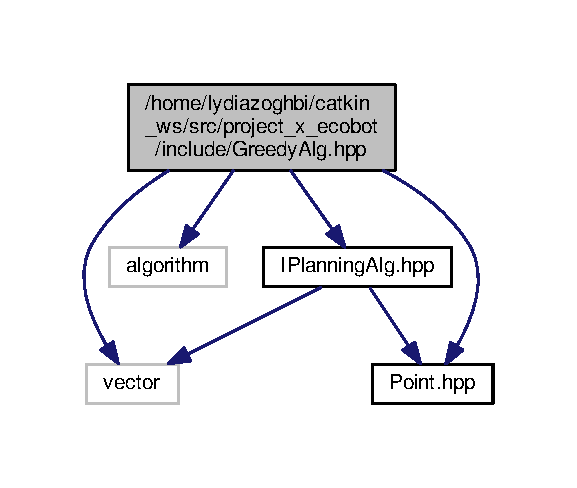
\includegraphics[width=277pt]{GreedyAlg_8hpp__incl}
\end{center}
\end{figure}
This graph shows which files directly or indirectly include this file\+:
\nopagebreak
\begin{figure}[H]
\begin{center}
\leavevmode
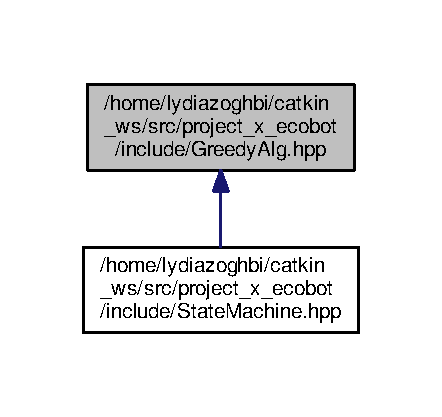
\includegraphics[width=212pt]{GreedyAlg_8hpp__dep__incl}
\end{center}
\end{figure}
\subsection*{Classes}
\begin{DoxyCompactItemize}
\item 
class \hyperlink{classGreedyAlg}{Greedy\+Alg}
\end{DoxyCompactItemize}


\subsection{Detailed Description}
Header file for \hyperlink{classGreedyAlg}{Greedy\+Alg} class. 

\begin{DoxyAuthor}{Author}
Lydia Zoghbi and Ryan Bates 
\end{DoxyAuthor}
\begin{DoxyCopyright}{Copyright}
Copyright Apache 2.\+0 License 
\end{DoxyCopyright}
\begin{DoxyDate}{Date}
12/09/2019 
\end{DoxyDate}
\begin{DoxyVersion}{Version}
1.\+0 
\end{DoxyVersion}

\hypertarget{ImageAnalysis_8hpp}{}\section{/home/lydiazoghbi/catkin\+\_\+ws/src/project\+\_\+x\+\_\+ecobot/include/\+Image\+Analysis.hpp File Reference}
\label{ImageAnalysis_8hpp}\index{/home/lydiazoghbi/catkin\+\_\+ws/src/project\+\_\+x\+\_\+ecobot/include/\+Image\+Analysis.\+hpp@{/home/lydiazoghbi/catkin\+\_\+ws/src/project\+\_\+x\+\_\+ecobot/include/\+Image\+Analysis.\+hpp}}


Header file for \hyperlink{classImageAnalysis}{Image\+Analysis} class.  


{\ttfamily \#include $<$math.\+h$>$}\\*
{\ttfamily \#include $<$cmath$>$}\\*
{\ttfamily \#include $<$vector$>$}\\*
{\ttfamily \#include $<$string$>$}\\*
{\ttfamily \#include $<$iostream$>$}\\*
{\ttfamily \#include $<$opencv2/highgui/highgui.\+hpp$>$}\\*
{\ttfamily \#include $<$opencv2/imgproc/imgproc.\+hpp$>$}\\*
{\ttfamily \#include $<$opencv2/imgcodecs/imgcodecs.\+hpp$>$}\\*
{\ttfamily \#include \char`\"{}Point.\+hpp\char`\"{}}\\*
Include dependency graph for Image\+Analysis.\+hpp\+:
\nopagebreak
\begin{figure}[H]
\begin{center}
\leavevmode
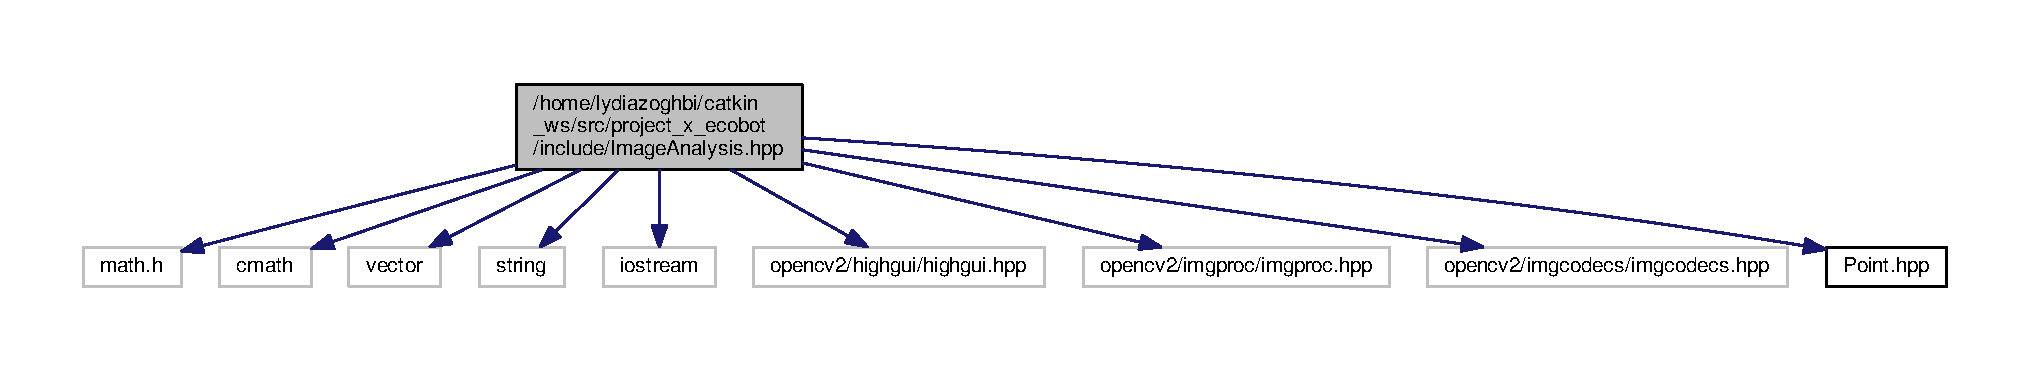
\includegraphics[width=350pt]{ImageAnalysis_8hpp__incl}
\end{center}
\end{figure}
This graph shows which files directly or indirectly include this file\+:
\nopagebreak
\begin{figure}[H]
\begin{center}
\leavevmode
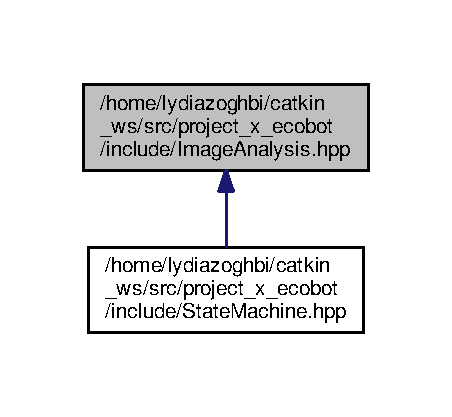
\includegraphics[width=217pt]{ImageAnalysis_8hpp__dep__incl}
\end{center}
\end{figure}
\subsection*{Classes}
\begin{DoxyCompactItemize}
\item 
class \hyperlink{classImageAnalysis}{Image\+Analysis}
\end{DoxyCompactItemize}


\subsection{Detailed Description}
Header file for \hyperlink{classImageAnalysis}{Image\+Analysis} class. 

\begin{DoxyAuthor}{Author}
Lydia Zoghbi 
\end{DoxyAuthor}
\begin{DoxyCopyright}{Copyright}
Copyright Apache 2.\+0 License 
\end{DoxyCopyright}
\begin{DoxyDate}{Date}
11/25/2019 
\end{DoxyDate}
\begin{DoxyVersion}{Version}
1.\+0 
\end{DoxyVersion}

\hypertarget{IPlanningAlg_8hpp}{}\section{/home/lydiazoghbi/catkin\+\_\+ws/src/project\+\_\+x\+\_\+ecobot/include/\+I\+Planning\+Alg.hpp File Reference}
\label{IPlanningAlg_8hpp}\index{/home/lydiazoghbi/catkin\+\_\+ws/src/project\+\_\+x\+\_\+ecobot/include/\+I\+Planning\+Alg.\+hpp@{/home/lydiazoghbi/catkin\+\_\+ws/src/project\+\_\+x\+\_\+ecobot/include/\+I\+Planning\+Alg.\+hpp}}
{\ttfamily \#include $<$vector$>$}\\*
{\ttfamily \#include \char`\"{}Point.\+hpp\char`\"{}}\\*
Include dependency graph for I\+Planning\+Alg.\+hpp\+:
\nopagebreak
\begin{figure}[H]
\begin{center}
\leavevmode
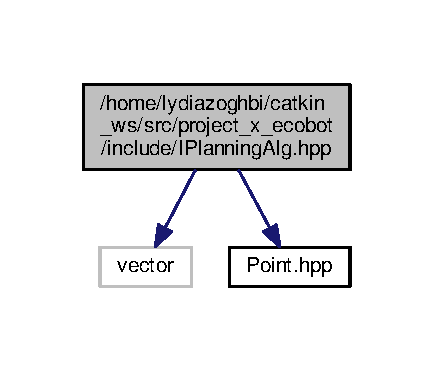
\includegraphics[width=208pt]{IPlanningAlg_8hpp__incl}
\end{center}
\end{figure}
This graph shows which files directly or indirectly include this file\+:
\nopagebreak
\begin{figure}[H]
\begin{center}
\leavevmode
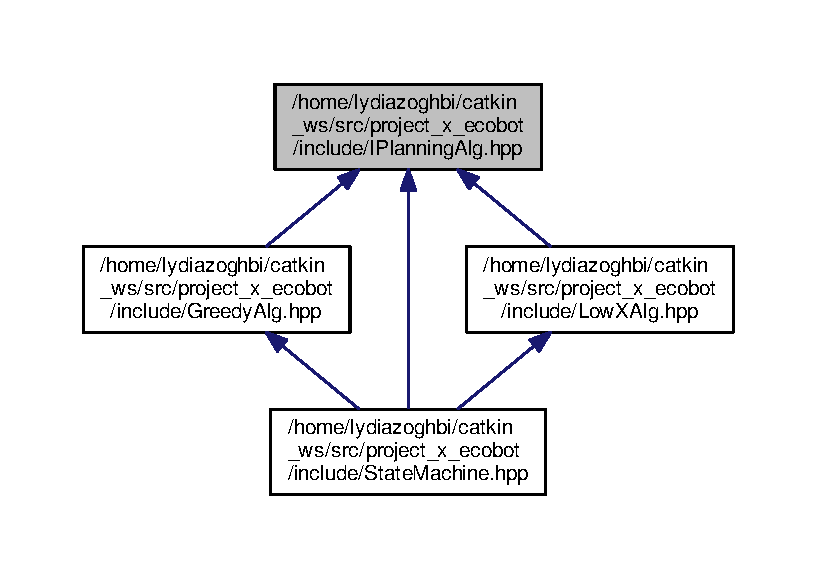
\includegraphics[width=350pt]{IPlanningAlg_8hpp__dep__incl}
\end{center}
\end{figure}
\subsection*{Classes}
\begin{DoxyCompactItemize}
\item 
class \hyperlink{classIPlanningAlg}{I\+Planning\+Alg}
\end{DoxyCompactItemize}

\hypertarget{LowXAlg_8hpp}{}\section{/home/lydiazoghbi/catkin\+\_\+ws/src/project\+\_\+x\+\_\+ecobot/include/\+Low\+X\+Alg.hpp File Reference}
\label{LowXAlg_8hpp}\index{/home/lydiazoghbi/catkin\+\_\+ws/src/project\+\_\+x\+\_\+ecobot/include/\+Low\+X\+Alg.\+hpp@{/home/lydiazoghbi/catkin\+\_\+ws/src/project\+\_\+x\+\_\+ecobot/include/\+Low\+X\+Alg.\+hpp}}


Header file for \hyperlink{classLowXAlg}{Low\+X\+Alg} class.  


{\ttfamily \#include $<$vector$>$}\\*
{\ttfamily \#include $<$algorithm$>$}\\*
{\ttfamily \#include \char`\"{}Point.\+hpp\char`\"{}}\\*
{\ttfamily \#include \char`\"{}I\+Planning\+Alg.\+hpp\char`\"{}}\\*
Include dependency graph for Low\+X\+Alg.\+hpp\+:
\nopagebreak
\begin{figure}[H]
\begin{center}
\leavevmode
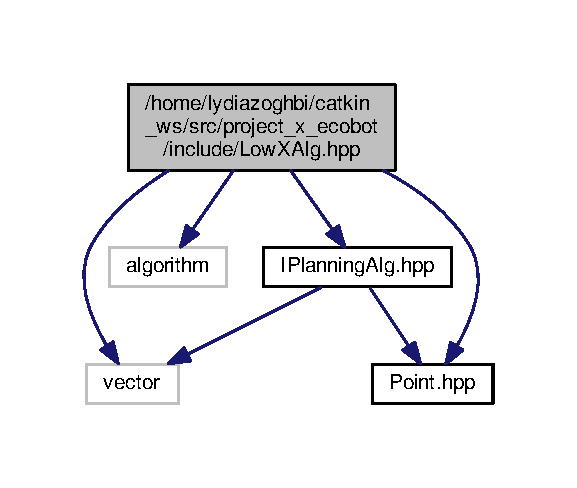
\includegraphics[width=277pt]{LowXAlg_8hpp__incl}
\end{center}
\end{figure}
This graph shows which files directly or indirectly include this file\+:
\nopagebreak
\begin{figure}[H]
\begin{center}
\leavevmode
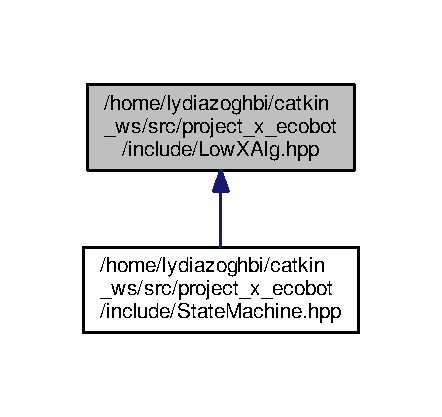
\includegraphics[width=212pt]{LowXAlg_8hpp__dep__incl}
\end{center}
\end{figure}
\subsection*{Classes}
\begin{DoxyCompactItemize}
\item 
class \hyperlink{classLowXAlg}{Low\+X\+Alg}
\end{DoxyCompactItemize}


\subsection{Detailed Description}
Header file for \hyperlink{classLowXAlg}{Low\+X\+Alg} class. 

\begin{DoxyAuthor}{Author}
Lydia Zoghbi and Ryan Bates 
\end{DoxyAuthor}
\begin{DoxyCopyright}{Copyright}
Copyright Apache 2.\+0 License 
\end{DoxyCopyright}
\begin{DoxyDate}{Date}
12/09/2019 
\end{DoxyDate}
\begin{DoxyVersion}{Version}
1.\+0 
\end{DoxyVersion}

\hypertarget{Point_8hpp}{}\section{/home/lydiazoghbi/catkin\+\_\+ws/src/project\+\_\+x\+\_\+ecobot/include/\+Point.hpp File Reference}
\label{Point_8hpp}\index{/home/lydiazoghbi/catkin\+\_\+ws/src/project\+\_\+x\+\_\+ecobot/include/\+Point.\+hpp@{/home/lydiazoghbi/catkin\+\_\+ws/src/project\+\_\+x\+\_\+ecobot/include/\+Point.\+hpp}}


Header file for \hyperlink{IPlanningAlg_8hpp}{I\+Planning\+Alg.\+hpp}.  


This graph shows which files directly or indirectly include this file\+:
\nopagebreak
\begin{figure}[H]
\begin{center}
\leavevmode
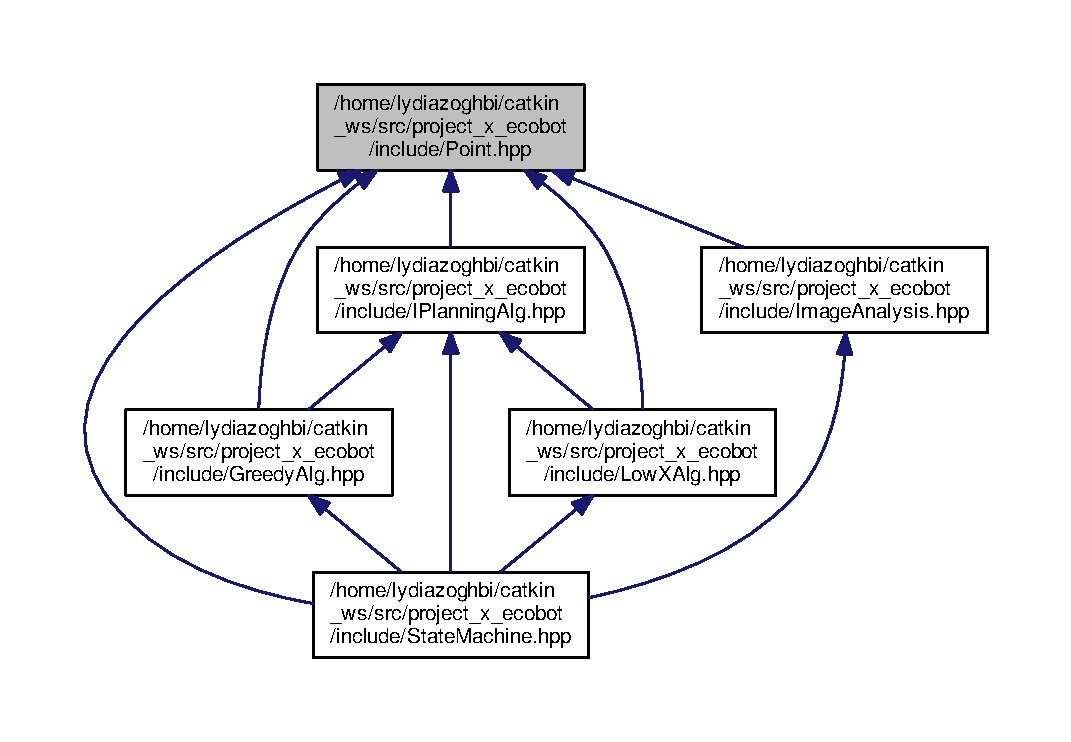
\includegraphics[width=350pt]{Point_8hpp__dep__incl}
\end{center}
\end{figure}
\subsection*{Classes}
\begin{DoxyCompactItemize}
\item 
class \hyperlink{classPoint}{Point}
\end{DoxyCompactItemize}


\subsection{Detailed Description}
Header file for \hyperlink{IPlanningAlg_8hpp}{I\+Planning\+Alg.\+hpp}. 

Header file for \hyperlink{classPoint}{Point} class.

\begin{DoxyAuthor}{Author}
Lydia Zoghbi and Ryan Bates 
\end{DoxyAuthor}
\begin{DoxyCopyright}{Copyright}
Copyright Apache 2.\+0 License 
\end{DoxyCopyright}
\begin{DoxyDate}{Date}
12/09/2019 
\end{DoxyDate}
\begin{DoxyVersion}{Version}
1.\+0 
\end{DoxyVersion}

\hypertarget{StateMachine_8hpp}{}\section{/home/lydiazoghbi/catkin\+\_\+ws/src/project\+\_\+x\+\_\+ecobot/include/\+State\+Machine.hpp File Reference}
\label{StateMachine_8hpp}\index{/home/lydiazoghbi/catkin\+\_\+ws/src/project\+\_\+x\+\_\+ecobot/include/\+State\+Machine.\+hpp@{/home/lydiazoghbi/catkin\+\_\+ws/src/project\+\_\+x\+\_\+ecobot/include/\+State\+Machine.\+hpp}}


Header file for \hyperlink{classStateMachine}{State\+Machine} class.  


{\ttfamily \#include $<$math.\+h$>$}\\*
{\ttfamily \#include $<$cv\+\_\+bridge/cv\+\_\+bridge.\+h$>$}\\*
{\ttfamily \#include $<$tf/transform\+\_\+datatypes.\+h$>$}\\*
{\ttfamily \#include $<$image\+\_\+transport/image\+\_\+transport.\+h$>$}\\*
{\ttfamily \#include $<$cmath$>$}\\*
{\ttfamily \#include $<$vector$>$}\\*
{\ttfamily \#include $<$string$>$}\\*
{\ttfamily \#include $<$memory$>$}\\*
{\ttfamily \#include $<$utility$>$}\\*
{\ttfamily \#include $<$iostream$>$}\\*
{\ttfamily \#include $<$algorithm$>$}\\*
{\ttfamily \#include \char`\"{}ros/ros.\+h\char`\"{}}\\*
{\ttfamily \#include \char`\"{}sensor\+\_\+msgs/\+Image.\+h\char`\"{}}\\*
{\ttfamily \#include \char`\"{}nav\+\_\+msgs/\+Odometry.\+h\char`\"{}}\\*
{\ttfamily \#include \char`\"{}geometry\+\_\+msgs/\+Twist.\+h\char`\"{}}\\*
{\ttfamily \#include $<$opencv2/highgui/highgui.\+hpp$>$}\\*
{\ttfamily \#include $<$opencv2/imgproc/imgproc.\+hpp$>$}\\*
{\ttfamily \#include $<$opencv2/imgcodecs/imgcodecs.\+hpp$>$}\\*
{\ttfamily \#include \char`\"{}Point.\+hpp\char`\"{}}\\*
{\ttfamily \#include \char`\"{}Low\+X\+Alg.\+hpp\char`\"{}}\\*
{\ttfamily \#include \char`\"{}Greedy\+Alg.\+hpp\char`\"{}}\\*
{\ttfamily \#include \char`\"{}I\+Planning\+Alg.\+hpp\char`\"{}}\\*
{\ttfamily \#include \char`\"{}Image\+Analysis.\+hpp\char`\"{}}\\*
Include dependency graph for State\+Machine.\+hpp\+:
\nopagebreak
\begin{figure}[H]
\begin{center}
\leavevmode
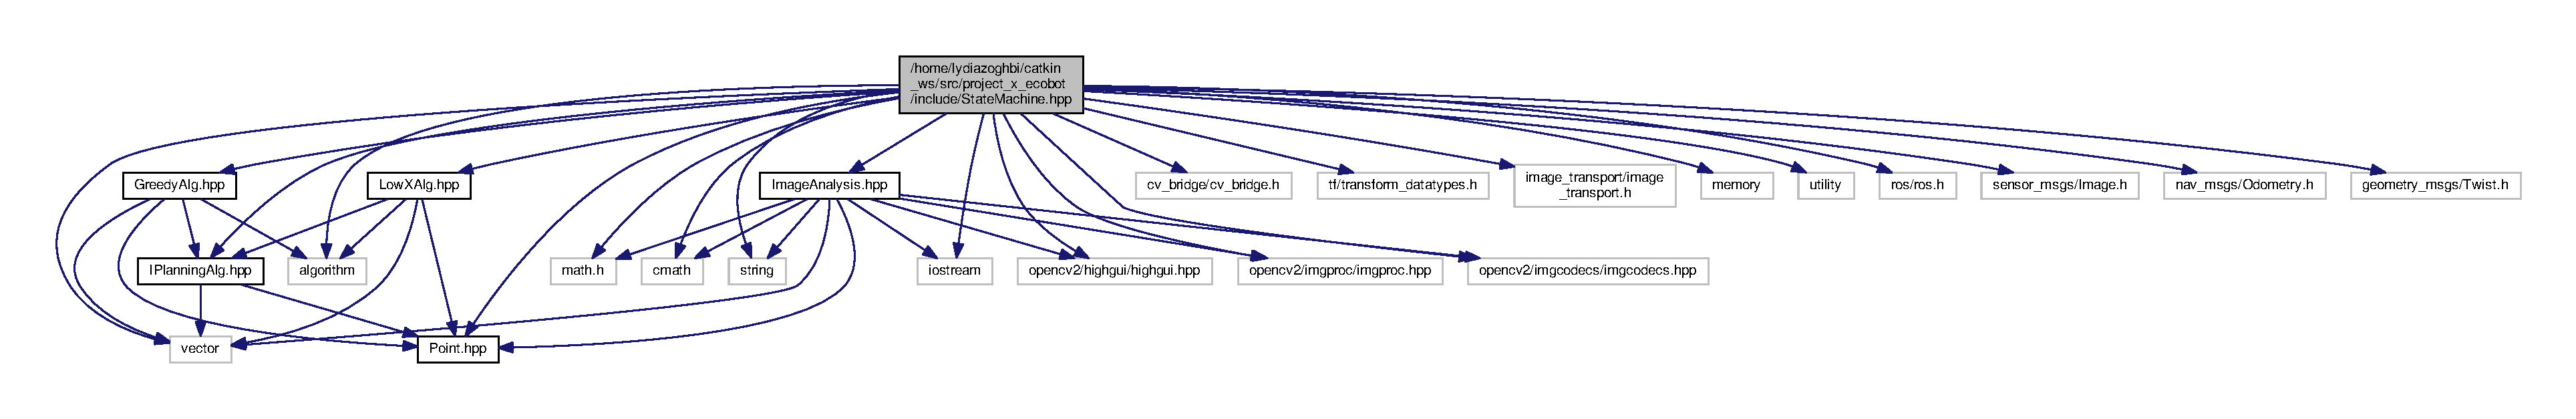
\includegraphics[width=350pt]{StateMachine_8hpp__incl}
\end{center}
\end{figure}
\subsection*{Classes}
\begin{DoxyCompactItemize}
\item 
class \hyperlink{classStateMachine}{State\+Machine}
\end{DoxyCompactItemize}


\subsection{Detailed Description}
Header file for \hyperlink{classStateMachine}{State\+Machine} class. 

\begin{DoxyAuthor}{Author}
Lydia Zoghbi and Ryan Bates 
\end{DoxyAuthor}
\begin{DoxyCopyright}{Copyright}
Copyright Apache 2.\+0 License 
\end{DoxyCopyright}
\begin{DoxyDate}{Date}
12/09/2019 
\end{DoxyDate}
\begin{DoxyVersion}{Version}
1.\+0 
\end{DoxyVersion}

%--- End generated contents ---

% Index
\backmatter
\newpage
\phantomsection
\clearemptydoublepage
\addcontentsline{toc}{chapter}{Index}
\printindex

\end{document}
